\section{Komponente eines Embedded Linux Systems}
\label{cha:tech_grund:sec:Komponente_eines_Emb_Lin_Sys}
In diesem Abschnitt möchte ich auf die wesentlichen Komponenten von eingebetteten Linux-Systemen im Detail eingehen. Im Anschluss daran wird der typische Boot-Prozess solcher Systeme beschrieben 
Fast Jedes embedded Linux Projekt beginnt mit der Erstellung, Konfiguration und Kompilierung der folgenden vier Komponenten \cite{Dervis2013}:
\begin{itemize}
	\item \textbf{Toolchain}: Die Toolchain enthält den Compiler und andere zur Erstellung von Code für Ihr Endgerät notwendige Werkzeuge
	\item \textbf{der Bootloader}: Beim Einschalten des Rechners, auf denen Linux als Betriebssystem installiert ist, wird nach der ersten Einrichtung ein Bootloader in den Speicher geladen und der Code ausgeführt. Die Hauptaufgabe des Bootloaders ist es, der Linux Kernel in den Speicher zu laden und dann es auszuführen. 
	\item \textbf{Der Kernel}: ist das Herzstück des Systems, das die Systemressourcen und Schnittstelle zur Hardware verwaltet.
	\item \textbf{Root filesystem}: beinhaltet die Bibliotheken und Programme, die ausgeführt werden, sobald der Kernel seine Initialisierung abgeschlossen hat.
\end{itemize}
Als Nächstes möchte ich den Boot-Prozess bei Systemen, die auf Zynq UltraScale+ MPSoCs basieren, erläutern, da dies genau die Plattform ist, die wir für unsere Arbeit verwenden werden. Die Abbildung ~\ref{fig:boot:process} zeit ein Beispiel für den Bootablauf an.

\begin{figure}[h]
	\begin{center}
		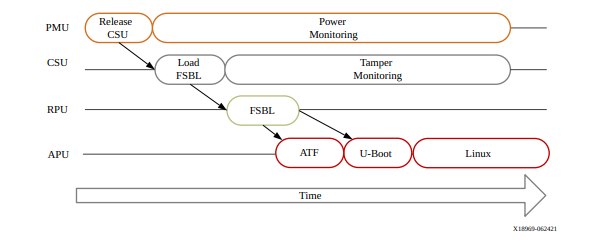
\includegraphics[width=1.1\textwidth]{./images/boot-flow.jpg}
	\end{center}
	\vspace{-5pt}
	\caption[der Bootvorgang bei zynq+MPSoCs]{Überblick über den Bootvorgang \cite{Xilinx2017}[p.~58]} % Eckige Klammer (optional): Caption-Text in Abbildungsverzeichnis
	\label{fig:boot:process}
	\vspace{-5pt}
\end{figure}

Der Bootvorgang bie Xilinx Bausteine besteht, ebenso wie bei allen Linux-Systemen, aus drei Phasen \cite{Xilinx2017}[p.~57], die von der Platform Management Unit (PMU) und die Configuration Security Unit (CSU) gesteuert und geführt wird. Das Booten des Geräts kann entweder im sicheren (\Fachbegriff{secure boot}) oder im nicht sicheren (\Fachbegriff{non-secure boot}) Modus durchgeführt werden 
\begin{itemize}
	\item \textbf{Pre-configuration stage (Oder Vor-Konfigurationsphase)}: Dieser Phase wird von der PMU angesteuert, die den PMU-ROM-Code zur Einrichtung des Systems ausführt. Die PMU wickelt alle Prozesse im Verbindung mit dem Zurücksetzen und Aufwachen ab.
	\item \textbf{Configuration stage oder (Konfiguration der Phase)}:Diese Phase übernimmt das Laden des First-Stage-Bootloader-Codes (FSBL) für den PS in das On-Chip-RAM (OCM), und zwar sowohl im sicheren als auch im unsicheren Boot-Modus. Während des Bootvorgangs lädt die CSU auch die PMU-Benutzerfirmware (PMU FW) in das PMU-RAM, um in Verbindung mit dem PMU-ROM Plattform-Management-Dienste bereitzustellen.
	\item \textbf{Post-configuration stage oder (Post-Konfigurationsphase)}: Nach dem Start der FSBL-Ausführung geht der CSU-ROM-Code in die Nachkonfigurationsphase über, die für die Reaktion auf Systemmanipulationen verantwortlich ist
\end{itemize}

auf dieser Ebene ist das Betriebssystem noch nicht vollständig betriebsbereit. sobald der FSBL an den TF-Agent übergeben wird, dann wird er Auf der Application processing units(APU) ausgeführt. TF-Agent wird an einen Second Stage Boot Loader wie U-Boot übergeben, der ein Betriebssystem wie Linux ausführt und lädt, und Linux lädt seinerseits die ausführbare Software.\\
Alle bisher genannten Linux-Komponenten, ob die Toolchains, der Bootloader, der Kernel oder das Root-Dateisystem können mit einem Build-System wie dem Yocto-Projekt erstellt werden. Da unser FPGA aber einen MPsoc enthält, der einen Bootloader, ATF-Firmware, pmufw, den Bitstream und u-boot benötigt, ist ein Build System zu verwenden, das automatisch alle diese Komponenten erzeugen kann.. Hierfür ist Petalinux am besten geeignet. Im nächsten Abschnitt werde ich das Petalinux Build System vorstellen. 


